\section{Lección \#1 - Conozcamos al triángulo rectángulo}
Cualquier estudiante de enseñanza media sabe que se trata de un triángulo que tiene un ángulo con amplitud $90\degree$. Sin embargo no muchos saben la cantidad de relaciones que se generan en ese polígono. Dediquemos entonces un tiempo al estudio de este triángulo tan ``generoso''.

\begin{multicols}{2}
    \begin{tikzpicture}[
      my angle/.style={
        every pic quotes/.append style={text=black},
        draw=white,
        angle radius=1cm,
      }]
      \coordinate [label=left:] (B) at (-2,-1.5);
      \coordinate [label=right:] (A) at (2,-1.5);
      \coordinate [label=above:] (C) at (-2,1.5);
      \draw (B) -- node[left] {$a$} (C) -- node[above] {$c$} (A) -- node[below] {$b$} (B);
      \draw (B) +(.25,0) |- +(0,.25);
      \pic [my angle, "$\alpha$"] {angle=C--A--B};
      \pic [my angle, "$\beta$"] {angle=B--C--A};
    \end{tikzpicture}
\columnbreak\\
1) \textbf{Teorema de Pitágoras}\\
\[c^2 = a^2 + b^2\]\\
2) \textbf{Razones Trigonométricas}
\begin{align*}
\sen\alpha &= \dfrac{a}{c}\\
\cos\alpha &= \dfrac{b}{c}\\
\tan\alpha &= \dfrac{a}{b}\\
\sen\alpha &= \cos\beta
\end{align*}
\end{multicols}

- Vea que basta conocer la longitud de dos lados o la amplitud de uno de los ángulos agudos y la longitud de uno de los tres lados para determinar el resto de los cinco elementos del triángulo.

\begin{multicols}{2}
    \begin{tikzpicture}[
      my angle/.style={
        every pic quotes/.append style={text=black},
        draw=white,
        angle radius=1cm,
      }]
     \coordinate [label=left:] (B) at (-2,-1.5);
      \coordinate [label=right:] (A) at (2,-1.5);
      \coordinate [label=above:] (C) at (-2,1.5);
      \coordinate [label=above:] (H) at (-0.56,0.42);
      
      \coordinate (F) at (-0.76,0.57);
      \coordinate (J) at (-0.91,0.37);
      \coordinate (K) at (-0.51,0.07);
      \coordinate (G) at (-0.36,0.27);
      
      \draw (F) -- (J);
      \draw (J) -- (K);
      \draw (K) -- (G);
      
      \draw (B) -- node[left] {$a$} (C);
      \draw (B) -- node[below] {$b$} (A);
      \draw (C) -- node[above] {$p$} (H);
      \draw (A) -- node[above] {$q$} (H);
      \draw (B) -- node[above] {$h$} (H);
    
      \pic [my angle, "$\alpha$"] {angle=C--A--B};
      \pic [my angle, "$\beta$"] {angle=B--C--A};
      \pic [my angle, "$\omega$"] {angle=H--B--C};
      \pic [my angle, "$\sigma$"] {angle=A--B--H};
    \end{tikzpicture}
\columnbreak\\
3) \textbf{Grupo de Teoremas de Pitágoras}
\vspace*{-0.1cm}
\begin{align*}
3.1)\hspace{1cm}h^2 &= p \cdot q\\
3.2)\hspace{1cm}a^2 &= c \cdot p\\
b^2 &= c \cdot q\\
3.3)\hspace{1cm}c^2 &= a^2 + b^2
\end{align*}
\end{multicols}

- Es suficiente conocer la longitud de dos de los seis segmentos determinados, o uno de ellos y uno de los cuatro ángulos determinados para calcular el valor del resto de los diez elementos

\subsubsection{Demostración de 3)}

Sean $\triangle_1$, $\triangle_2$ y $\triangle_3$ de lados $(a,h,p)$, $(a,b,c)$ y $(b,h,q)$ tenemos:
\begin{equation*}
 \left.\begin{aligned}
        \triangle_1 \sim \triangle_2 &: \dfrac{a}{c}=\dfrac{h}{b}=\dfrac{p}{a} \Longrightarrow a^2 = c \cdot p\\
    \triangle_2 \sim \triangle_3 &: \dfrac{b}{c}=\dfrac{h}{a}=\dfrac{q}{b} \Longrightarrow b^2 = c \cdot q
       \end{aligned}
 \right\}
 \qquad \textbf{3.2) Teorema de los catetos}
\end{equation*}
\hspace{1.3cm}$\triangle_1 \sim \triangle_3: \dfrac{a}{b}=\dfrac{h}{q}=\dfrac{p}{h} \Longrightarrow h^2 = p \cdot q$\hspace{0.1cm} \qquad \textbf{3.1) Teorema de la altura}\\

Sumando las dos ecuaciones obtenidas en $3.2$:
\begin{align*}
    a^2 + b^2 &= c \cdot p + c \cdot q\\
              &= c (p + q)\\
              &= c \cdot c\\
              &= c^2 \qquad\qquad\qquad\qquad\qquad\qquad\qquad\textbf{3.3) Teorema de Pitágoras}
\end{align*}

Vea además que el área del triángulo podemos expresarla como:
\begin{center}
$A = \dfrac{ab}{2}$ y $A = \dfrac{ch}{2}$ $\Longrightarrow$ $\dfrac{ab}{c} = h$    
\end{center}

Vea también que $\sigma = \beta$ y $\omega = \alpha$ por ser ángulos agudos con lados respectivamente perpendiculares

\begin{multicols}{2}
4)\vspace*{-0.5cm}\\
\hspace*{0.9cm}
    \begin{tikzpicture}
      \coordinate [label=left:$C$] (B) at (-2,-1.5);
      \coordinate [label=right:$B$] (A) at (2,-1.5);
      \coordinate [label=above:$A$] (C) at (-2,1.5);
      \coordinate [label=above:$M$] (H) at (0,0);
    %   \draw (B) -- node[left] {$a$} (C) -- node[above] {$c$} (A) -- node[below] {$b$} (B);
      \draw (B) -- node[left] {} (C);
      \draw (B) -- node[below] {} (A);
      \draw (C) -- node[above] {} (H);
      \draw (A) -- node[above] {} (H);
      \draw (B) -- node[above] {} (H);
    %   \draw (H) +(-.25,0) |- +(0,.25);
    \end{tikzpicture}
\columnbreak\\

Sea $M$ punto medio de $\overline{AB}$

$\Longrightarrow \overline{AM} = \overline{MB} = \overline{CM}$
\begin{center}
\textbf{Teorema de la mediana de la\\ hipotenusa}
\end{center}
\end{multicols} 

\subsubsection{Demostración}
\begin{itemize}
    \item[$\cdot\hspace{0.05cm}\text{-})$] Sea $\overline{MH}\perp\overline{CB}$ en $H \Longrightarrow \overline{MH}$ es la paralela media de $\overline{AC}$\\
\hspace*{2cm}$\therefore \overline{MH}$ es altura y mediana de $\overline{BC}$ en $\triangle CMB$\\
\hspace*{2cm}o sea, $\triangle CMB$ es isósceles de base $\overline{CB}$, etc...

    \item[$\cdot\hspace{0.05cm}\text{-})$] Sea $D$ un punto de la prolongación de $\overline{CM}$; $\overline{CM} =\overline{MD} \Longrightarrow ACBD$ es paralelogramo-rectángulo y $\overline{AM}=\overline{MB}=\overline{CM}=\overline{MD}$ por propiedades de un triángulo

    \item[$\cdot\hspace{0.05cm}\text{-})$] $M$ es circuncentro del $\triangle ABC \Longrightarrow \overline{AM}=\overline{MB}=\overline{MC}=$ radio de la circunferencia de centro $M$ que pasa por $A$, $B$ y $C$ (recíproco del teorema de Tales)
\end{itemize}


\noindent5) En todo triángulo rectángulo con un ángulo agudo de $30\degree$ tenemos:
\begin{itemize}
    \item[i)]El cateto opuesto al ángulo de $30\degree$ mide la longitud de la hipotenusa dividida por dos ($a = c \div 2$) 
    \item[ii)]El cateto adyacente al ángulo de $30\degree$ mide $\sqrt{3}$ veces la longitud del cateto opuesto al ángulo de $30\degree$ ($b = \sqrt{3}a$)
\end{itemize}

\subsubsection{Demostración}
\begin{multicols}{2}
    \begin{tikzpicture}[
      my angle/.style={
        every pic quotes/.append style={text=black},
        draw=white,
        angle radius=1cm
      }]
      \coordinate [label=left:] (A) at (0,4);
      \coordinate [label=left:] (B) at (0,0);
      \coordinate [label=above:] (C) at (3.46,2);
      \coordinate [label=left:] (M) at (0,2);
      \draw[dashed] (B) -- node[left] {$a$} (M);
      \draw (M) -- node[left] {$a$} (A);
      \draw (M) -- node[above] {$b$} (C);
      \draw (A) -- node[above] {$c$} (C);
      \draw[dashed] (C) -- node[below] {$c$} (B);
      \draw (M) +(.25,0) |- +(0,.25);
      \draw (M) +(.25,0) |- +(0,-0.25);
      \pic [my angle, "$60\degree$"scale=0.8] {angle=M--A--C};
      \pic [my angle, "$60\degree$"scale=0.8] {angle=C--B--M};
      \pic [my angle, "$30\degree$"scale=0.8] {angle=A--C--M};
      \pic [my angle, "$30\degree$"scale=0.8] {angle=M--C--B};
    \end{tikzpicture}
\columnbreak\\
\noindent Reflejando el triángulo dado de lados $(a,b,c)$ sobre el cateto $b$ obtengo un triángulo equilátero\\
$\Longrightarrow$ i) $a = \dfrac{c}{2}$\\
\hspace*{0.7cm}ii) $b = \sqrt{3}a$ (por Teo. de Pitágoras)\\

\noindent nota: De aquí se obtienen las razones trigonométricas de los ángulos $30\degree$ y $60\degree$
\end{multicols} 


\noindent6) En todo triángulo rectángulo e isósceles tenemos:
\begin{itemize}
    \item[] La longitud de la hipotenusa es igual a $\sqrt{2}$ veces la longitud de los catetos ($c = \sqrt{2}s$) Esto es resultado de aplicar teorema de Pitágoras con $a=b$
    \item[] nota: de aquí se obtienen las razones trigonométricas del ángulo de $45\degree$
\end{itemize}


\noindent\textbf{*} 7) En todo triángulo rectángulo, la suma de la longitud del inradio y el circunradio es igual a la media aritmética de los catetos.

\subsubsection{Demostración}
\begin{multicols}{2}
    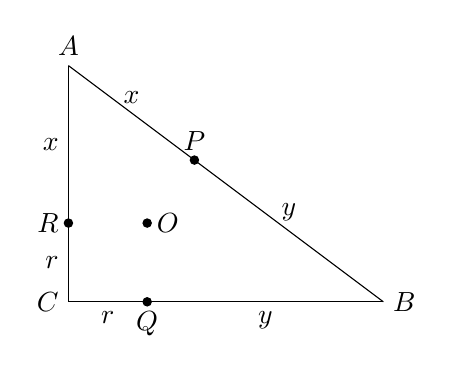
\begin{tikzpicture}
        \coordinate [label=left:$C$] (C) at (-2,-1.5);
        \coordinate [label=right:$B$] (B) at (2,-1.5);
        \coordinate [label=above:$A$] (A) at (-2,1.5);
        \coordinate [label=above:$P$] (P) at (-0.4,0.3);
        \coordinate [label=below:$Q$] (Q) at (-1,-1.5);
        \coordinate [label=left:$R$] (R) at (-2,-0.5);
        \coordinate [label=right:$O$] (O) at (-1,-0.5);
            
        \draw (A) -- node[left] {$x$} (R);
        \draw (R) -- node[left] {$r$} (C);
        \draw (C) -- node[below] {$r$} (Q);
        \draw (Q) -- node[below] {$y$} (B);
        \draw (B) -- node[above] {$y$} (P);
        \draw (P) -- node[above] {$x$} (A);
              
        \filldraw (O) circle[radius=1.5pt];
        \filldraw (P) circle[radius=1.5pt];
        \filldraw (Q) circle[radius=1.5pt];
        \filldraw (R) circle[radius=1.5pt];
      
    \end{tikzpicture}
\columnbreak\\
\noindent Sean $P$, $Q$, $R$ puntos de tangencia del incírculo del $\triangle ABC$ con los lados $\overline{AB}$, $\overline{BC}$, $\overline{CA}$, tenemos:
\begin{itemize}
    \item[] $\overline{AR}=\overline{AP}=x$
    \item[] $\overline{RC}=\overline{CQ}=r$ (inradio)
    \item[] $\overline{PB}=\overline{QB}=y$
\end{itemize}
\end{multicols} 

\begin{equation*}
    \begin{aligned}
        \Longrightarrow a &= \overline{CQ} + \overline{QB} = r + y\\
        b &= \overline{AR} + \overline{RC} = x + r\\
        c &= \overline{AP} + \overline{PB} = x + y = \text{diámetro del circuncírculo}\\
        \Longrightarrow a +b &= r + y + x + r = 2R + 2r\\
        \Longrightarrow r + R &= \dfrac{a+b}{2} 
    \end{aligned}
\end{equation*}

8) , 9). 10), ... pueden ser sugerencias de los lectores a este humilde trabajo.


\section{Lección \#2 - Rectas y Puntos Notables}
lección 2

\section{Lección \#3 - Circunferencia y Cuadrilátero}
Antes de proseguir quiero señalar que esto no es un compendio sobre temas de nuestra enseñanza, mi mayor anhelo es colaborar con la cultura matemática sobre todo con notas poco publicadas y que sean muy interesantes...

\vspace{0.5cm}
\noindent 1) Ya vimos que en todo triángulo puede inscribirse y circunscribirse una circunferencia. Sin embargo este privilegio no lo poseen los cuadriláteros. Para que una circunferencia pueda circunscribirse en un cuadrilátero $ABCD$ tiene que cumplirse que los ángulos opuestos sean suplementarios ($\measuredangle A + \measuredangle C = 180\degree$, $\measuredangle B + \measuredangle D = 180\degree$), este cuadrilátero es llamado Cuadrilátero Cíclico ($CC$).

\hspace{2cm} y para que pueda ser inscrito tiene que cumplir que $\overline{AB}+\overline{CD} = \overline{BC}+\overline{DA}$ (Teorema de Pitot).

\vspace{0.5cm}
Conocer esto es muy ventajoso, pues veamos...

\vspace{0.5cm}
\noindent\parbox[][][t]{.3\linewidth}{
    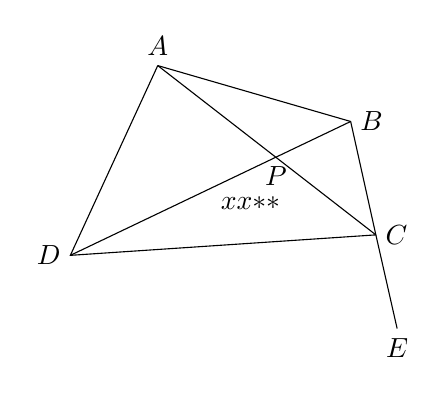
\begin{tikzpicture}
      \coordinate [label=above:$A$] (A) at (-0.8,1.83);
      \coordinate [label=right:$B$] (B) at (1.65,1.12);
      \coordinate [label=right:$C$] (C) at (1.97,-0.32);
      \coordinate [label=left:$D$] (D) at (-1.91,-0.58);
      \coordinate [label=below:$E$] (E) at (2.24,-1.51);
      
      \coordinate [label=below:$P$] (P) at (0.7,0.67);
      \coordinate (O) at (0,0);
      
      \draw (A) -- (B) -- (C) -- (D) -- (A);
      \draw (A) -- (C);
      \draw (D) -- (B);
      \draw (C) -- (E);
     
      \tkzLabelAngle[pos=0.3](D,A,C){$x$}; 
      \tkzLabelAngle[pos=0.3](D,B,C){$x$}; 
      \tkzLabelAngle[pos=0.4](A,B,D){$*$}; 
      \tkzLabelAngle[pos=0.4](A,C,D){$*$}; 
      \tkzMarkAngle[size=0.5cm,arc=l,mark=none](B,D,A);
      \tkzMarkAngle[size=0.5cm,arc=l,mark=none](B,C,A);
      \tkzMarkAngle[size=0.8cm,arc=ll,mark=none](C,A,B);
      \tkzMarkAngle[size=0.8cm,arc=ll,mark=none](C,D,B);
      
      \tkzDrawCircle(O,A);
    \end{tikzpicture}
}
\parbox[][][t]{.03\linewidth}{\hspace{.03\linewidth}}
\parbox[][][t]{.67\linewidth}{
 Sea $ABCD$ un $CC$ tal que sus diagonales se cortan en $P \Longrightarrow$
 \begin{itemize}
     \item[i $\cdot\hspace{0.05cm}\text{-}$] $\measuredangle ABD = \measuredangle ACD$, $\measuredangle DBC = \measuredangle DAC$, etc
     \item[ii $\cdot\hspace{0.05cm}\text{-}$] $\measuredangle DAB = \measuredangle DCE$ (siendo $B$, $C$ y $E$ alineados)
     \item[iii $\cdot\hspace{0.05cm}\text{-}$] $\overline{AP}\cdot\overline{PC} = \overline{DP}\cdot\overline{PB}$ (potencia de un punto PP)
     \item[iv $\cdot\hspace{0.05cm}\text{-}$] $\overline{AB}\cdot\overline{CD} + \overline{BC}\cdot\overline{DA} = \overline{AC}\cdot\overline{BD}$ (Teorema de Ptolomeo)
     \item[v $\cdot\hspace{0.05cm}\text{-}$] $A_{ABCD} = \sqrt{p(p-a)(p-b)(p-c)(p-d)}$ ($p$ semiperímetro)
 \end{itemize}
}

\noindent y muchas otras relaciones, y como sabemos, la Geometría es el arte de relacionar elementos de las figuras presentadas.

\vspace{0.5cm}
\noindent 2) Potencia de un punto: Puede presentarse de varias formas, ver que en 1.iii $\triangle APB \sim \triangle CPD$, esta sería la primera forma.

\vspace{0.5cm}
forma 2)


\noindent\parbox[][][t]{.3\linewidth}{
    \begin{tikzpicture}
      \coordinate [label=left:$A$] (A) at (-1.91, -0.58);
      \coordinate [label=below right:$B$] (B) at (2, 0.02);
      \coordinate [label=right:$C$] (C) at (3.02,0.17);
      \coordinate [label=above right:$D$] (D) at (1.24, 1.57);
      \coordinate (E) at (0.29,2.32);
      
      \coordinate (O) at (0,0);
      
      \draw (A) -- (B) -- (C) -- (D) -- (A);
      \draw[dashed] (D) -- (B);
      \draw (D) -- (E);
   
      \tkzMarkAngle[size=0.8cm,arc=l,mark=none](C,A,D);
      \tkzMarkAngle[size=0.8cm,arc=l,mark=none](B,D,C);
   
      \tkzDrawCircle(O,A);
    \end{tikzpicture}
}
\parbox[][][t]{.2\linewidth}{\hspace{.03\linewidth}}
\parbox[][][t]{.5\linewidth}{
 Si $\overline{CD}$ tangente en $D$\\
 $\Longrightarrow \overline{DC}^2 = \overline{AC}\cdot\overline{BC}$\\
 Vea que  $\triangle ACD \sim \triangle DBC$
}

\newpage
forma 3)
\vspace{0.3cm}

\noindent\parbox[][][t]{.3\linewidth}{
    \begin{tikzpicture}
      \coordinate [label=above left:$A$] (A) at (-1.54,1.28);
      \coordinate [label=below left:$B$] (B) at (-0.5,-1.94);
      \coordinate [label=below:$C$] (C) at (-0.2,-2.85);
      \coordinate [label=below right:$D$] (D) at (0.31,-1.98);
      \coordinate [label=above right:$E$] (E) at (1.87,0.7);
      
      \coordinate (O) at (0,0);
      
      \draw (A) -- (B) -- (C) -- (D) -- (E);
      \draw[dashed] (E) -- (B);
      \draw[dashed] (A) -- (D);
      
      \tkzMarkAngle[size=1.5cm,arc=l,mark=none](C,A,D);
      \tkzMarkAngle[size=1.5cm,arc=l,mark=none](B,E,C);
   
      \tkzDrawCircle(O,A);
    \end{tikzpicture}
}
\parbox[][][t]{.2\linewidth}{\hspace{.03\linewidth}}
\parbox[][][t]{.5\linewidth}{
 $\overline{CE}\cdot\overline{DC} = \overline{CA}\cdot\overline{BC}$\\
 Vea que  $\triangle ACD \sim \triangle BCE$
}

\vspace{0.3cm}

\noindent 3) Eje radical de dos circunferencias ($ER$)

Veamos las formas de presentarse

\vspace{0.5cm}

\noindent\parbox[][][t]{.45\linewidth}{
forma 1

\begin{center}
Circunferencias Tangentes\\
Externas    
\end{center}

\vspace{0.5cm}

    \begin{tikzpicture}
      \coordinate [label=below:$O_1$] (O1) at (-2.5, 0);
      \coordinate [label=below:$O_2$] (O2) at (2, 0);
      \coordinate [label=below:] (P) at (-1,0);
      \coordinate [label=below right:] (E) at (-1,2.5);
      \coordinate [label=below:$ER$] (R) at (-1,-3);
      
      \filldraw (O1) circle[radius=1.5pt];
      \filldraw (O2) circle[radius=1.5pt];
      
      \draw[dashed] (O1) -- (O2);
      \draw (E) -- (R);
      
      \tkzMarkRightAngle(O1,P,E);
      
      \tkzDrawArc[angles,color=black](O1,P)(-90,150)
      \tkzDrawArc[angles,color=black](O2,P)(100,-80)
    \end{tikzpicture}
}
\parbox[][][t]{.1\linewidth}{\hspace{.1\linewidth}}
\noindent\parbox[][][t]{.45\linewidth}{
forma 2

\begin{center}
Circunferencias\\
Exteriores    
\end{center}

\vspace{0.5cm}

    \begin{tikzpicture}
      \coordinate [label=below:$O_1$] (O1) at (-2.5, 0);
      \coordinate [label=below:$O_2$] (O2) at (2, 0);
      \coordinate [label=below:] (P) at (-1,0);
      \coordinate [label=below:] (P1) at (-1.5,0);
      \coordinate [label=below:] (P2) at (-0.8,0);
      \coordinate [label=below right:] (E) at (-1,2.5);
      \coordinate [label=below:$ER$] (R) at (-1,-3);
      
      \filldraw (O1) circle[radius=1.5pt];
      \filldraw (O2) circle[radius=1.5pt];
      
      \draw[dashed] (O1) -- (O2);
      \draw (E) -- (R);
      
      \tkzMarkRightAngle(O1,P,E);
      
      \tkzDrawArc[angles,color=black](O1,P1)(-140,150)
      \tkzDrawArc[angles,color=black](O2,P2)(70,-60)
    \end{tikzpicture}
}

\vspace{0.5cm}

\noindent\parbox[][][t]{.45\linewidth}{
forma 3

\begin{center}
Circunferencias Tangentes\\
Interiores    
\end{center}

\vspace{0.5cm}

    \begin{tikzpicture}
      \coordinate [label=below:$O_1$] (O1) at (0.1, 0);
      \coordinate [label=below:$O_2$] (O2) at (1.5, 0);
      \coordinate [label=below:] (P) at (-1.5,0);
      \coordinate [label=below right:] (E) at (-1.5,3);
      \coordinate [label=below:$ER$] (R) at (-1.5,-3);
      
      \filldraw (O1) circle[radius=1.5pt];
      \filldraw (O2) circle[radius=1.5pt];
      
      \draw[dashed] (O2) -- (P);
      \draw (E) -- (R);
      
      \tkzMarkRightAngle(O1,P,E);
      
      \tkzDrawCircle(O1,P);
      \tkzDrawCircle(O2,P);
    \end{tikzpicture}
}
\parbox[][][t]{.1\linewidth}{\hspace{.1\linewidth}}
\noindent\parbox[][][t]{.45\linewidth}{
forma 4

\begin{center}
Circunferencias\\
Secantes    
\end{center}

\vspace{0.5cm}

    \begin{tikzpicture}
      \coordinate [label=below:$O_1$] (O1) at (-3, 0);
      \coordinate [label=below:$O_2$] (O2) at (1, 0);
      \coordinate [label=below:] (P) at (-1.68,0);
      \coordinate [label=right:$A$] (A) at (-1.68,1.54);
      \coordinate [label=right:$B$] (B) at (-1.68,-1.54);
      \coordinate [label=below right:] (E) at (-1.68,3.5);
      \coordinate [label=below:$ER$] (R) at (-1.68,-3);
      
      \coordinate [label=below right:$P$] (PP) at (-1.68,3);
      \coordinate [label=below:$Q$] (QQ) at (-3.95,1.79);
      \coordinate [label=below:$T$] (TT) at (0.89,3.09);
      
      \filldraw (O1) circle[radius=1.5pt];
      \filldraw (O2) circle[radius=1.5pt];
      \filldraw (QQ) circle[radius=1.5pt];
      \filldraw (TT) circle[radius=1.5pt];
      
      \draw[dashed] (O1) -- (O2);
      \draw (E) -- (R);
      \draw (QQ) -- (PP);
      \draw (PP) -- (TT);
      
      \tkzMarkRightAngle(O1,P,E);
      
      \tkzDrawArc[angles,color=black](O1,A)(-140,150)
      \tkzDrawArc[angles,color=black](O2,A)(70,-60)
    \end{tikzpicture}
}

\vspace{0.5cm}

En cada forma vemos que $ER \perp O_1O_2$, pero lo más destacado es que: Todo punto situado en el $ER$ tiene la misma potencia respecto a ambas circunferencias. Vea como ejemplo en la forma 4 $\overline{PQ}^2 = \overline{PB}\cdot\overline{PA}=\overline{PT}^2$, siendo $\overline{PQ}$ y $\overline{PT}$ tangentes. 

\vspace{0.5cm}

\noindent 4) Centro radical de 3 circunferencias ($CR$).


\vspace{0.5cm}

\noindent\parbox[][][t]{.45\linewidth}{
    \begin{tikzpicture}
    \coordinate [label=left:$O_1$] (O1) at (-4, 1);
    \coordinate [label=right:$O_2$] (O2) at (0.48, 4.36);
    \coordinate [label=below:$O_3$] (O3) at (-0.32, -0.52);
    
    \coordinate [label=below:] (R1) at (-2.72, 1.9);
    \coordinate [label=below:] (R2) at (-1.72, 2.34);
    \coordinate [label=below:] (R3) at (-1.54, 0.74);
    
    \coordinate [label=above right:$CR$] (CR) at (-1.68, 1.61);
    
    \coordinate [label=above:$ER$] (ER11) at (-3.48,4.01);
    \coordinate [label=below:] (ER12) at (-0.96, 0.65);
    
    \coordinate [label=below:$ER$] (ER21) at (-2.76,-1.01);
    \coordinate [label=below:] (ER22) at (-1.34, 2.44);
    
    \coordinate [label=below:$ER$] (ER31) at (2.3,0.96);
    \coordinate [label=below:] (ER32) at (-2.41, 1.73);
    
    \filldraw (CR) circle[radius=1.5pt];
    
    \draw[dashed] (O1) -- (O2) -- (O3) -- (O1);
    \draw (ER11) -- (ER12);
    \draw (ER21) -- (ER22);
    \draw (ER31) -- (ER32);
      
    \tkzDrawCircle(O1,R1);
    \tkzDrawArc[angles,color=black](O2,R2)(150,300)
    \tkzDrawArc[angles,color=black](O3,R3)(-5,200)
    \end{tikzpicture}
}
\parbox[][][t]{.1\linewidth}{\hspace{.1\linewidth}}
\noindent\parbox[][][t]{.45\linewidth}{
\vfill
\begin{center}
Es el punto\\
donde concurren\\
los tres $ER$
\end{center}
\vfill
}


\vspace{0.8cm}

\noindent 5) Teorema de Ptolomeo


\section{Lección \#4 - Otros Teoremas}
Estas notas van dirigidas mayormente a estudiantes de Alto Rendimiento que se preparan con esmero para enfrentar las diferentes competencias convocadas por las matemáticas.

$1\hspace{-0.05cm}\cdot\hspace{-0.05cm}\text{-}$ En todo $\triangle$ se cumple que: $a+b>c$, $b+c>a$, $c+a>b \longrightarrow$ Teorema de la desigualdad triangular.

$2\hspace{-0.05cm}\cdot\hspace{-0.05cm}\text{-}$ En todo $\triangle$ se cumple que: el segmento que une los puntos medios de dos de sus lados es paralelo al tercero y mide su mitad $\longrightarrow$ Teorema de la paralela media de un $\triangle$.

$3\hspace{-0.05cm}\cdot\hspace{-0.05cm}\text{-}$ Si dos bisectrices de un $\triangle$ tienen igual longitud $\Longrightarrow$ el $\triangle$ es isósceles $\longrightarrow$ Teorema de Steiner

$4\hspace{-0.05cm}\cdot\hspace{-0.05cm}\text{-}$ La suma de las distancias desde un punto interior de un $\triangle$ equilátero a los lados del $\triangle$ es $=$ a la longitud de su altura $\longrightarrow$ Teorema de Viviani

$5\hspace{-0.05cm}\cdot\hspace{-0.05cm}\text{-}$ Si sobre los lados $\overline{AB}$ y $\overline{AC}$ de un $\triangle ABC$ se construyen, por fuera, los $\triangle$ equiláteros $ABC'$ y $CAB' \Longrightarrow \overline{BB'} = \overline{CC'}$

$6\hspace{-0.05cm}\cdot\hspace{-0.05cm}\text{-}$ Si $G$ es el baricentro de un $\triangle ABC$ y por $G$ se traza una recta que corte a los 3 lados $\Longrightarrow \overline{AX} + \overline{BZ} = \overline{CY}$, siendo $\overline{AX}$, $\overline{BZ}$ y $\overline{CY}$ perpendiculares desde $A$, $B$, $C$ a la recta.

$7\hspace{-0.05cm}\cdot\hspace{-0.05cm}\text{-}$ Las proyecciones de un punto de una circunferencia sobre los lados de un $\triangle$ inscrito en dicha circunferencia determinan una recta $\longrightarrow$ Recta de Simpson.

$8\hspace{-0.05cm}\cdot\hspace{-0.05cm}\text{-}$ Circunferencia de los 9 puntos $\longrightarrow$ Es la que pasa por los puntos medios de cada lado, los pies de las alturas y los puntos medios de los segmentos que unen los vértices al ortocentro de un $\triangle$. El centro de esta circunferencia es el punto medio desde el ortocentro al centro de la circunferencia circunscrita.

$9\hspace{-0.05cm}\cdot\hspace{-0.05cm}\text{-}$ Triángulo pedal $\longrightarrow$ Es el $\triangle$ determinado por los pies de las alturas de un $\triangle$. El ortocentro del $\triangle$ coincide con el incentro del $\triangle$ pedal.

$ 10\hspace{-0.05cm}\cdot\hspace{-0.05cm}\text{-} $ Teorema de Stewart: Sea $\overline{AD} $ una ceviana cualquiera...

\noindent\parbox[][][t]{.4\linewidth}{
    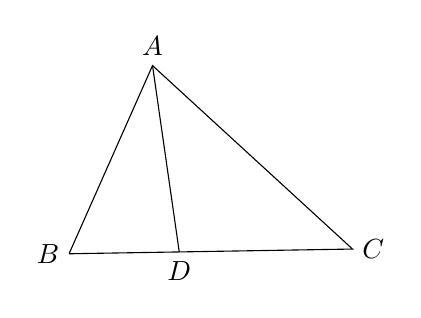
\begin{tikzpicture}
      \coordinate [label=left:$B$] (B) at (0,0);
      \coordinate [label=right:$C$] (C) at (3.6,0.06);
      \coordinate [label=above:$A$] (A) at (1.06,2.39);
      \coordinate [label=below:$D$] (D) at (1.4,0.02);
      \draw (B) -- (C) -- (A) -- (B);
      \draw (A) -- (D);
    \end{tikzpicture}
}
\parbox[][][t]{.05\linewidth}{\hspace{.05\linewidth}}
\parbox[][][t]{.55\linewidth}{
 $\overline{AB}^2\cdot\overline{DC} + \overline{AC}^2\cdot\overline{BD} = \overline{AD}^2\cdot\overline{BC} + \overline{BD}\cdot\overline{DC}\cdot\overline{BC}$
 
 \vspace{0.4cm}
 
 Para su demostración, trace la altura desde $A$ y aplique reiteradas veces el teorema de Pitágoras
 
}

\vspace{0.4cm}

$ 11\hspace{-0.05cm}\cdot\hspace{-0.05cm}\text{-} $  ???? bisectriz interior y exterior de un $\triangle$

\noindent\parbox[][][t]{.32\linewidth}{
    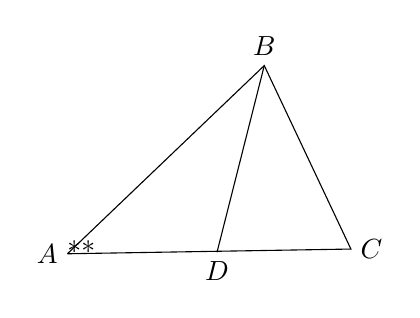
\begin{tikzpicture}
      \coordinate [label=left:$A$] (A) at (0,0);
      \coordinate [label=right:$C$] (C) at (3.6,0.06);
      \coordinate [label=above:$B$] (B) at (2.5,2.39);
      \coordinate [label=below:$D$] (D) at (1.9,0.02);
      
      \draw (A) -- (C) -- (B) -- (A);
      \draw (B) -- (D);
      \tkzLabelAngle[pos=0.5](A,B,D){$*$};
      \tkzLabelAngle[pos=0.5](D,B,C){$*$};
    \end{tikzpicture}
}
\parbox[][][t]{.15\linewidth}{$\dfrac{\overline{AB}}{\overline{BC}}=\dfrac{\overline{AD}}{\overline{DC}}$}
\parbox[][][t]{.53\linewidth}{
 \begin{tikzpicture}
      \coordinate [label=left:$A$] (A) at (0,0);
      \coordinate [label=above:$B$] (B) at (3.68,1.82);
      \coordinate [label=below:$C$] (C) at (3.9,0);
      
      \coordinate [label=below:$D$] (D) at (7.05,0);
      \coordinate [label=left:] (E) at (4.75,2.35);
      \draw (A) -- (C) -- (B) -- (A);
      \draw (B) -- (D);
      \draw[dashed] (C) -- (D);
      \draw[dashed] (B) -- (E);
      \tkzLabelAngle[pos=0.5](C,B,D){$*$};
      \tkzLabelAngle[pos=0.4](D,B,E){$*$};
    \end{tikzpicture}
}


\newpage

$ 12\hspace{-0.05cm}\cdot\hspace{-0.05cm}\text{-} $  Teorema de Ceva y Menelao

\noindent\parbox[][][t]{.35\linewidth}{
    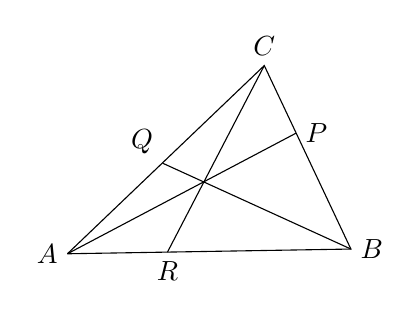
\begin{tikzpicture}
      \coordinate [label=left:$A$] (A) at (0,0);
      \coordinate [label=right:$B$] (B) at (3.6,0.06);
      \coordinate [label=above:$C$] (C) at (2.5,2.39);
      
      \coordinate [label=above left:$Q$] (Q) at (1.21,1.15);
      \coordinate [label=right:$P$] (P) at (2.9,1.53);
      \coordinate [label=below:$R$] (R) at (1.27,0.02);
      
      \draw (A) -- (B) -- (C) -- (A);
      \draw (A) -- (P);
      \draw (B) -- (Q);
      \draw (C) -- (R);
      
    \end{tikzpicture}
}
\parbox[][][t]{.2\linewidth}{$\dfrac{\overline{AR}}{\overline{RB}}\cdot\dfrac{\overline{BP}}{\overline{PC}}\cdot\dfrac{\overline{CQ}}{\overline{QA}}=1$}
\parbox[][][t]{.45\linewidth}{
    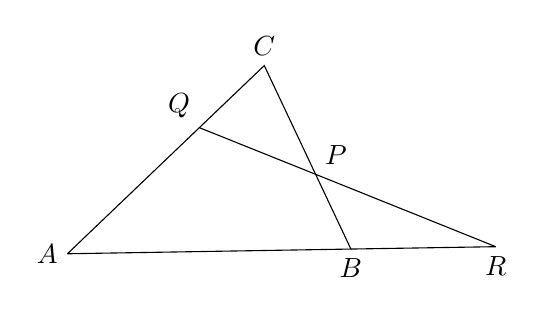
\begin{tikzpicture}
      \coordinate [label=left:$A$] (A) at (0,0);
      \coordinate [label=below:$B$] (B) at (3.6,0.06);
      \coordinate [label=above:$C$] (C) at (2.5,2.39);
      
      \coordinate [label=above left:$Q$] (Q) at (1.68,1.6);
      \coordinate [label=above right:$P$] (P) at (3.15,1.01);
      \coordinate [label=below:$R$] (R) at (5.44,0.09);
      
      \draw (A) -- (B) -- (C) -- (A);
      \draw (B) -- (R);
      \draw (Q) -- (P) -- (R);
      
      
    \end{tikzpicture}
}

 \vspace{0.4cm}
 
$ 13\hspace{-0.05cm}\cdot\hspace{-0.05cm}\text{-} $ Teorema de Pascal: En todo hexágono inscriptible sin lados opuestos paralelos, las intersecciones de los lados opuestos determinan 3 puntos alineados

$ 14\hspace{-0.05cm}\cdot\hspace{-0.05cm}\text{-} $ Desigualdad de Euler: $R \ge 2r$ con igualdad si el $\triangle$ es equilátero. $R \rightarrow $ circunradio, $r \rightarrow$ inradio

$ 15\hspace{-0.05cm}\cdot\hspace{-0.05cm}\text{-} $ Cálculo de áreas:
\begin{itemize}
    \item[-] $\triangle$ : $A = \dfrac{b\cdot h}{2}= \dfrac{a\cdot b \sen \gamma}{2} = \rho r = \dfrac{abc}{4R} = \sqrt{\rho(\rho-a)(\rho-b)(\rho-c)}$ (Herón)\vspace{0.4cm}\\
    $a$, $b$, $c$ lados del $\triangle$, $h \rightarrow$ altura del lado $b$\\
    $\gamma \rightarrow$ ángulo opuesto al lado $c$\\
    $\rho \rightarrow$ semiperímetro del $\triangle$
    
    \item[-] Cuadrilátero: $A = \dfrac{d_1 \cdot d_2}{2} \sen \sigma $\vspace{0.4cm}\\
    $d_1$, $d_2 \rightarrow$ diagonales, \hspace{0.5cm}$\sigma \rightarrow \measuredangle$ formado por las diagonales
\end{itemize}

$ 16\hspace{-0.05cm}\cdot\hspace{-0.05cm}\text{-} $  En todo paralelogramo la suma de los cuadrados de sus lados multiplicados por dos es $=$ a la suma de los cuadrados de sus diagonales.

$ 17\hspace{-0.05cm}\cdot\hspace{-0.05cm}\text{-} $ Teorema de Varignon: Al unir los 4 puntos medios de cada lado de un cuadrilátero se obtiene un paralelogramo.

\begin{center}
    \texttt{Algunos lemas necesarios}
\end{center}

$ 18\hspace{-0.05cm}\cdot\hspace{-0.05cm}\text{-} $  La distancia del circuncentro a uno de los lados de un $\triangle$ tiene la mitad de la longitud del segmento que une al ortocentro del $\triangle$ con el vértice opuesto al lado.

$ 19\hspace{-0.05cm}\cdot\hspace{-0.05cm}\text{-} $ Si $\overline{AB} \perp \overline{CD}$ en $N \Longrightarrow \overline{AC}^2 = \overline{AD}^2  = \overline{BC}^2 = \overline{BD}^2$

$ 20\hspace{-0.05cm}\cdot\hspace{-0.05cm}\text{-} $ Si $\overline{AA_1} \perp \overline{BB_1} \Longrightarrow a^2 + b^2 = 5c^2$, con $\overline{AA_1}$ mediana de $a$ y $\overline{BB_1}$ mediana de $b$ en un $\triangle ABC$ (Esto se prueba aplicando 19)

$ 21\hspace{-0.05cm}\cdot\hspace{-0.05cm}\text{-} $ Lema de Raví: En $\triangle ABC$, $I$ es el incentro, $P$, $Q$, $R$ puntos de tangencia del incírculo con los lados del $\triangle \Longrightarrow$

\noindent\parbox[][][t]{.35\linewidth}{
    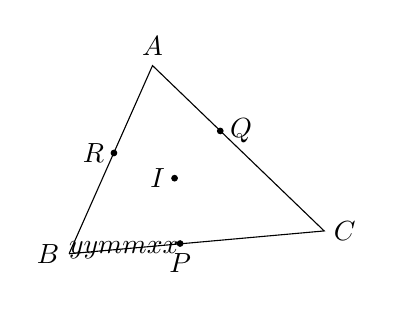
\begin{tikzpicture}
      \coordinate [label=left:$B$] (B) at (0,0);
      \coordinate [label=right:$C$] (C) at (3.24,0.29);
      \coordinate [label=above:$A$] (A) at (1.06,2.39);
      
      \coordinate [label=below:$P$] (P) at (1.41,0.13);
      \coordinate [label=right:$Q$] (Q) at (1.92,1.56);
      \coordinate [label=left:$R$] (R) at (0.57,1.28);
      
      \coordinate [label=left:$I$] (I) at (1.34,0.96);
      
      \draw (B) -- (C) -- (A) -- (B);
      
      \filldraw (I) circle[radius=1pt];
      \filldraw (P) circle[radius=1pt];
      \filldraw (Q) circle[radius=1pt];
      \filldraw (R) circle[radius=1pt];
      
      \tkzLabelSegment[left=1pt](B,R){$y$};  
      \tkzLabelSegment[below=1pt](B,P){$y$};
      
      \tkzLabelSegment[below=1pt](C,P){$m$};
      \tkzLabelSegment[right=1pt](C,Q){$m$};
      
      \tkzLabelSegment[left=1pt](A,R){$x$};
      \tkzLabelSegment[right=1pt](A,Q){$x$};
      
    \end{tikzpicture}
}
\parbox[][][t]{.05\linewidth}{\hspace{.05\linewidth}}
\parbox[][][t]{.6\linewidth}{
 $\overline{AR} = \overline{AQ} = x$, $\overline{BR} = \overline{BP} = y$, $\overline{CP} = \overline{CQ} = m$
 
\vspace{0.4cm}

 $\therefore a = y + m$, $b = m + x$, $c = x + y$

\vspace{0.4cm}
 
 $\Longrightarrow m = \dfrac{1}{2}(a+b-c)$, $y = \dfrac{1}{2}(c+b-b)$, $x = \dfrac{b+c-a}{2}$
}

\vspace{0.4cm}

$ 22\hspace{-0.05cm}\cdot\hspace{-0.05cm}\text{-} $ 


\noindent\parbox[][][t]{.49\linewidth}{
    \begin{tikzpicture}[scale=0.8]
      \coordinate [label=left:$T$] (T) at (-4,0);
      \coordinate [label=above right:$A$] (A) at (2.54,3.09);
      \coordinate [label=below:$B$] (B) at (1.51,-3.7);
      
      \coordinate [label=right:] (OI) at (-1.44,0);
      \coordinate [label=above:] (OE) at (0,0);
      
      \coordinate [label=right:$\omega$] (EI) at (1.12,0);
      \coordinate [label=left:$\Gamma$] (EE) at (4,0);
      
      \coordinate [label=above:$E$] (E) at (-1.77,2.54);
      \coordinate [label=below:$F$] (F) at (-2.26,-2.42);
      
      \coordinate [label=below:$A_1$] (A1) at (0.18,1.98);
      \coordinate [label=above:$B_1$] (B1) at (-0.47,-2.37);
      
      \tkzDrawCircle(OI,T);
      \tkzDrawCircle(OE,T);
      
      \draw (A) -- (T) -- (B) -- (A);
      \draw (A) -- (E);
      \draw (B) -- (F);
      
      \filldraw (E) circle[radius=1pt];
      \filldraw (F) circle[radius=1pt];
      \filldraw (A1) circle[radius=1pt];
      \filldraw (B1) circle[radius=1pt];
      
      
    \end{tikzpicture}
}
\parbox[][][t]{.51\linewidth}{
 Si $\omega$ y $\Gamma$ son dos circunferencias tangentes internas en $T$; $A$ y $B$ son puntos de $\Gamma$,\\$A_1 = \overline{TA} \bigcap \omega$ y $B_1 = \overline{TB} \bigcap \Gamma \Longrightarrow$
 
\vspace{0.4cm}
 
 \hspace{0.5cm}$\dfrac{\overline{TA}}{\overline{TB}}=\dfrac{\overline{AE}}{\overline{BF}}$ siendo $\overline{AE}$ y $\overline{BF}$ tangentes a $\omega$
 
\vspace{0.4cm}
 
 
 - Vea que $\overline{A_1B_1} \parallel \overline{AB}$\\y por potencia de un punto
 \begin{equation*}
     \begin{aligned}
      \overline{AE}^2 &= \overline{AA_1} \cdot \overline{AT}\\
      \overline{BF}^2 &= \overline{BB_1} \cdot \overline{BT}\text{, etc ...}
     \end{aligned}
 \end{equation*}
}

\vspace{0.4cm}

$ 23\hspace{-0.05cm}\cdot\hspace{-0.05cm}\text{-} $ 


\noindent\parbox[][][t]{.55\linewidth}{
    \begin{tikzpicture}[scale=0.8]
      \coordinate [label=above:$A$] (A) at (0.37,2.35);
      \coordinate [label=left:$B$] (B) at (-3.38,-1.4);
      \coordinate [label=right:$C$] (C) at (2.28,-1.4);
      
      \coordinate [label=below:$D$] (D) at (0,-1.4);
      \coordinate [label=right:$E$] (E) at (1.25,0.63);
      \coordinate [label=left:$F$] (F) at (-0.99,0.99);
      
      \coordinate [label=below left:$X$] (X) at (-1.1,-1.4);
      \coordinate [label=left:$Y$] (Y) at (3.78,-4.35);
      \coordinate [label=right:$Z$] (Z) at (-5.54,-3.58);
      
      
      \coordinate [label=below right:$T$] (T) at (0,1.4);
      \coordinate [label=right:$\sigma$] (O) at (0,0);
      
      \coordinate [label=right:$\sigma_a$] (Oa) at (-1.14,-7);
      
      \coordinate [label=right:] (P) at (-5.99, -4.01);
      \coordinate [label=right:] (Q) at (4.1,-4.98);
      
      \draw (B) -- (C) -- (A) -- (B);
      \draw (A) -- (P);
      \draw (A) -- (Q);
      \draw (T) -- (O) -- (D);
      \draw (A) -- (T) -- (X);
      \draw (Oa) -- (X);
      
      
      \filldraw (O) circle[radius=1.5pt];
      \filldraw (Z) circle[radius=1.5pt];
      \filldraw (Y) circle[radius=1.5pt];
      \filldraw (Oa) circle[radius=1.5pt];
    
    \tkzDrawCircle(O,T);
      
    \end{tikzpicture}
}
%\parbox[][][t]{.01\linewidth}{\hspace{.01\linewidth}}
\parbox[][][t]{.45\linewidth}{
 Si $D$, $E$, $F$ puntos de tangencia del incírculo de centro $\sigma$ en $\triangle ABC$. Si $\overline{DT}$ es diámetro; recta $\overrightarrow{AT}$ corta $BC$ en $X \Longrightarrow \overline{BD} = \overline{CX}$
 
 \vspace{0.4cm}
 
 Demostración:\vspace{0.1cm} \\$2 \overline{BD} = \overline{BC} + \overline{AB} - \overline{AC}$ por $21)$\\
 $= \overline{BF} + \overline{BZ} + \overline{XD}$\\
 $= \overline{FZ} + \overline{XD} = \overline{EY} + \overline{XD}$\\
 $= \overline{EC} + \overline{CY} + \overline{XD} = \overline{DC} + \overline{XC} + \overline{XD}$\\
 $= 2 \overline{CX}$
 
 \vspace{0.4cm}
 
 $Z$ y $Y$ puntos de tangencia del excírculo de $A$ con lados $\overrightarrow{AB}$ y $\overrightarrow{AC}$
}

\vspace{0.4cm}


\vspace{1cm}

24, 25, 26 ... pueden ser sugerencias de los amigos de la matemática.



\section{Lección \#5}
Comenzamos con la entrega de notas relacionadas con la Teoría de Números (TN) y el álebra. Aquí va a haber para todos los gustos, desde notas trilladas en nuestra enseñanza media hasta notas necesarias para alumnos de alto rendimiento.

\vspace{0.5cm}

$1\hspace{-0.05cm}\cdot\hspace{-0.05cm}\text{-}$ Un \# cualquiera puede expresarse en el sistema decimal como suma de potencias de base $10$. Por ejemplo: $\overline{abc}=100a + 10b + c$, $\overline{abcd}= 1000a + 100b + 10c + d$

\vspace{0.5cm}

$2\hspace{-0.05cm}\cdot\hspace{-0.05cm}\text{-}$ Un \# lo llamamos Cuadrado Perfecto cuando su raíz cuadrada es un número entero $(0, 1, 4, 9, 16, ..., n^2)$. Vea que la diferencia de dos (CP) consecutivos es igual a la suma de las raices cuadradas de ambos \# ejemplo: $49-36=13=7+6$

\vspace{0.5cm}

$3\hspace{-0.05cm}\cdot\hspace{-0.05cm}\text{-}$ Múltiplos y Divisores de un \#. Ejemplo: Múltiplos de $6$: $0,6,12,18,...$ Divisores de $24$: $1, 2, 3, 4, 6, 8, 24$.

\vspace{0.5cm}

$4\hspace{-0.05cm}\cdot\hspace{-0.05cm}\text{-}$ Números Primos: Son los que poseen $2$ divisores $(2,3,5,7,11,13,...)$. Números Primos entre sí: Son aquellos que solo tienen al uno como divisor común. Ejemplo: $3$ y $10$, $11$ y $17$, $4$ y $9$, $5$, $8$ y $21$ ... 

\vspace{0.5cm}

$5\hspace{-0.05cm}\cdot\hspace{-0.05cm}\text{-}$ Máximo Común Divisor (\texttt{mcd}): De todos los divisores comunes de dos o varios \#, el mayor es el \texttt{mcd}. Ejemplo: $\texttt{mcd}(24,32)=8$.

Mínimo Común Múltiplo (\texttt{mcm}): De todos los múltiplos comunes de dos o varios \#, el menor es el \texttt{mcm}. Ejemplo: $\texttt{mcm}(8,10)=40$

¿Cómo determinar el (\texttt{mcd}) y el (\texttt{mcm}) entre varios números?

Ejemplo: Sean $A=30600$, $B=4340$, $C=2674200$

\hspace{1.6cm}o sea $A=2^3\cdot5^2\cdot7\cdot19$, $B=2^2\cdot5\cdot7\cdot31$, $C=2^4\cdot5^3\cdot19^2\cdot37$

$\Longrightarrow \texttt{mcd}(A,B,C)=2^2\cdot5=20$ (Vea que se toman solo las bases comunes de las potencias elevadas al menor exponente)

\hspace{.8cm}$\texttt{mcd}(B,C)=2^2\cdot5=20$

\hspace{.8cm}$\texttt{mcd}(A,C)=2^3\cdot5^2\cdot19=3800$

\hspace{.8cm}$\texttt{mcm}(A,B,C)=2^4\cdot5^3\cdot7\cdot19^2\cdot31\cdot37$ (Vean que se toman todas las bases de las potencias y entre las comunes la de mayor exponente)

\hspace{.8cm}$\texttt{mcm}(A,B)=2^3\cdot5^2\cdot7\cdot19\cdot31$

\vspace{0.5cm}

$6\hspace{-0.05cm}\cdot\hspace{-0.05cm}\text{-}$ Reglas de divisibilidad: Un \# es divisible por ...
\begin{itemize}
    \addtolength{\itemindent}{1cm}
    \item[$2 -$] si su última cifra es par o es $= 0$
    \item[$5 -$] si su última cifra es $0$ o $5$
    \item[$10 -$] si su última cifra es $= 0$
    \item[$3 -$] si al sumar todas sus cifras se obtiene un múltiplo de $3$
    \item[$9 -$] si al sumar todas sus cifras se obtiene un múltiplo de $9$
    \item[$4 -$] si las dos últimas cifras del \# conforman un múltiplo de $4$
    \item[$8 -$] si las tres últimas cifras del \# conforman un múltiplo de $8$
    \item[$11 -$] cuando al restar los dos resultados de sumar las cifras de orden par y las de orden impar, se obtiene un múltiplo de 11, veamos... \vspace{-0.3cm}
    \item[] $\overline{abcde}$\hspace{.65cm}$S_1=b+d$\hspace{.65cm}$S_2=a+c+d$\hspace{.65cm}$|S_1 - S_2| = 11k$
    \item[$6 -$] cuando es divisible por $2$ y $3$ a la misma vez
    \item[$12 -$] cuando es divisible por $3$ y $4$ a la misma vez
    \item[$15 -$] cuando es divisible por $3$ y $5$ a la misma vez
    \item[$36 -$] cuando es divisible por $4$ y $9$ a la misma vez
    \item[] Vea que $2$ y $3$, $3$ y $4$, $3$ y $5$, $4$ y $9$ son \# primos entre sí\vspace{-0.3cm}
    \item[] Ejemplo: $1536$ es divisible por: $1,2,3,4,6,8,12,...,1536$ \vspace{-0.3cm}
    \item[]\hspace{2.5cm}no es divisible por: $5,10,9,11,36,...$
    \item[$7 -$] cuando separamos su última cifra y multiplicándola por $2$, dicho resultado se le resta al \# que resultó de suprimir la última cifra al \# original, obteniendo un múltiplo de $7$\vspace{-0.3cm}
    \item[] Ejemplo: $51492$ : $2\cdot2=4$, $5149-4=5145$, $5\cdot2=10$, $514-10=504$, $4\cdot2=8$\vspace{-0.3cm}
    \item[] $50-8=42$ $\Longrightarrow 51492$ es múltiplo de $7$
\end{itemize}

Ahora existe una regla general que nos permite obtener la regla de divisibilidad de cualquier \# primo. En cualquier caso debemos separar la última cifra del \# y multiplicarlo por un \#n $n$ y luego realizar el mismo algoritmo que la regla del $7$. El problema es ver quién es $n$.

Debemos buscar qué dígitos multiplicados por el \# al cual le estamos investigando la regla de divisibilidad , da como resultado un \# cuya última cifra es $= 1$. Del resultado de este producto nos interesa solo las cifras que queden a la izquierda del $1$, y este será el valor de $n$.

Ejemplo Regla del $97$: $97\cdot3=291 \Longrightarrow n=29$
% \vspace{-0.3cm}

\hspace{1cm}Sea $12804$: $4\cdot29=116$, $1280-116=1164$, $4\cdot29=116$, $116-116=0$

$\Longrightarrow 12804$ es divisible por $97$
\begin{center}
    \texttt{$-\cdot-\cdot-$}
\end{center}
$7\hspace{-0.05cm}\cdot\hspace{-0.05cm}\text{-}$ Divisibilidad: El número natural $n$ es un divisor del número natural $m$ si existe $x \in \mathbb{N}$ tal que $m = nx$ y se escribe $n \mid m$ o $m$ $\vdots$ $n$. Se lee $n$ divide a $m$ o $m$ es múltiplo de $n$
\begin{itemize}
    \def\labelitemi{-}
    \addtolength{\itemindent}{1cm}
    \item Para todo $n \in \mathbb{Z}_+$ ; $1 \mid n$ y $n \mid n$
    \item Si $a \mid b$ y $a \mid c \Longrightarrow a \mid b \pm c$
    \item Si $a \mid b \Longrightarrow a \mid bc$ ; $\forall c \in \mathbb{Z}$
    \item Si $a \mid b$ y $b \mid c \Longrightarrow a \mid c$
    \item Si $a \mid b$ y $a \mid c \Longrightarrow a \mid (bx + cy)$ $\forall x,y \in \mathbb{Z}$ 
    \item Si $a \mid b$ y $b \mid a \Longrightarrow a = \pm b$ 
    \item Si $a \mid b$, $a > 0$ , $b > 0 \Longrightarrow b \ge a$
    \item Dado un polinomio $P=p^{\alpha_1} \cdot p^{\alpha_2} \cdot p^{\alpha_3} \cdot\cdot\cdot\cdot p^{\alpha_n}$ decimos que la cantidad de divisores $D$ de $P$ es $D=(\alpha_1 + 1)(\alpha_2 + 1)(\alpha_3 + 1) \cdot\cdot\cdot\cdot (\alpha_n + 1)$
    \item Sea $p$ primo tal que $p \mid ab \Longrightarrow p \mid a$ o $p \mid b$
    \item Todo \# primo mayor que $3$ puede expresarse como $4n \pm 1$; $6k \pm 1$ con $n, k \in \mathbb{N}^*$
\end{itemize}

\vspace{0.5cm}

$8\hspace{-0.05cm}\cdot\hspace{-0.05cm}\text{-}$ \texttt{mcd} y \texttt{mcm}. Conveniemos que $(a,b) = \texttt{mcd}(a,b)$ y $[a,b]= \texttt{mcm}(a,b)$
\begin{itemize}
    \def\labelitemi{-}
    \addtolength{\itemindent}{1cm}
    \item Si $a \mid b$ y $a \mid c \Longrightarrow a \mid (b,c)$
    \item $(ma, mb) = m(a,b)$ $\forall m \in \mathbb{Z}_+$, $a,b \in \mathbb{N}$
    \item $(a,b)=(a \pm b, a) = (b, b \pm a)$
    \item Si $(m,n) = d \Longrightarrow m = ad, n= bd$; $a,b \in \mathbb{Z}$, $(a,b) = 1$
    \item $(a,b) = \dfrac{ab}{[a,b]}$ y $[a,b,c] = \dfrac{(a,b,c)\cdot abc}{(a,b)(b,c)(c,a)}$
\end{itemize}

\vspace{0.5cm}

$9\hspace{-0.05cm}\cdot\hspace{-0.05cm}\text{-}$ Congruencia: Sean $a,b \in \mathbb{Z}$, $m \in \mathbb{N}^* \Longrightarrow$ ``$a$'' es congruente con ``$b$'' módulo ``$m$'' ($a \equiv b$ $($mod $m)$) si $a$ y $b$ dejan el mismo resto al dividirlos por ``$m$''
\begin{itemize}
    \def\labelitemi{-}
    \addtolength{\itemindent}{1cm}
    \item $a \equiv b$ $($mod $m) \Longleftrightarrow a - b$ es divisible por $m$
    \item Si $a,b,c,d,k \in \mathbb{N}^*$, $n \in \mathbb{N}$ y $a \equiv b$, $c \equiv d$ $($mod $m) \Longrightarrow$
        \begin{itemize}
            \addtolength{\itemindent}{1cm}
            \item[$\cdot$] $a+c \equiv b+d$, $a-c \equiv b-d$, $ac \equiv bd$, $ka \equiv kb$ $($mod $m)$
            \item[$\cdot$] $a^n \equiv b^n$ $($mod $m)$
            \item[$\cdot$] $a:k \equiv b:k$ $($mod $m)$ si $(k,m)=1$ y $a = kc$ y $b = kd$
        \end{itemize}
    \item $a \equiv a$ $($mod $m)$
    \item Si $a \equiv b$ $\Longrightarrow$ $b \equiv a$ $($mod $m)$
    \item Si $a \equiv b$ y $b \equiv c \Longrightarrow a \equiv c$ $($mod $m)$
    \item Si $a \equiv b$ $($mod $m) \Longrightarrow (a,m) \equiv (b,m)$ $($mod $m)$
    \item Si $ax \equiv ay$ $($mod $m)$ y $(a,m) = 1 \Longrightarrow x \equiv y$  $($mod $m)$
\end{itemize}


\vspace{0.5cm}

$9\hspace{-0.05cm}\cdot\hspace{-0.05cm}\text{-}$ Teorema de Fermat: Sea $p$ primo y $n \in \mathbb{N} \Longrightarrow n^p \equiv n$ $($mod $p)$

\hspace{0.7cm}Pequeño teorema de Fermat:

\hspace{0.9cm} Sea $p$ primo, $a \in \mathbb{Z}_+$; $p \nmid a \Longrightarrow a^{p-1} \equiv 1$ $($mod $p)$

\vspace{0.5cm}

\hspace{0.7cm}Teorema de Euler: Sean $a,m \in \mathbb{N}$; $(a,m) = 1 \Longrightarrow a^{\phi(m)} \equiv 1$ $($mod $m)$ donde $\phi(m)$ es el indicador y nos da la cantidad de \# primos con $m$, no mayores que él tal que $\phi(p) = p-1$ siendo $p$ primo.

\vspace{0.5cm}

\vspace{1cm}

11, 12, 13, ..., pueden ser sugerencias de los amigos lectores.


\section{Lección \#6}
El álgebra es una de las disciplinas insigneas dentro del estudio de las matemáticas. En estas notas tenemos en cuenta el trabajo con polinomios, ecuaciones, desigualdades y funciones entre tantas líneas que contempla este tema.

\vspace{0.5cm}

$1\hspace{-0.05cm}\cdot\hspace{-0.05cm}\text{-}$ Productos Notables:
\begin{itemize}
    \def\labelitemi{-}
    \addtolength{\itemindent}{0.5cm}
    \item[] A los más conocidos incorporamos estos de gran aplicación
    \item $(a \pm b)^3 = a^3 \pm 3a^2b + 3ab^ \pm b^3$
    \item $(a+b+c)^2 = a^2 + b^2 + c^2 + 2ab + 2bc + 2ca$
    \item $(a+b+c)^3 = a^3 + b^3 + c^3 + 3a^2b + 3a^2c + 3ab^2 + 3b^2c + 3ac^2 + 3bc^2 + 6abc$
    \item $(a+b)(b+c)(c+a) = a^2b +a^2c + ab^2 + b^2c + ac^2 + bc^2 + 2abc$
\end{itemize}

\vspace{0.5cm}

$2\hspace{-0.05cm}\cdot\hspace{-0.05cm}\text{-}$ Factorización: Al factor común, diferencia de cuadrados y trinomio agregamos otras formas...
\begin{itemize}
    \def\labelitemi{-}
    \addtolength{\itemindent}{0.5cm}
    \item Factor común por agrupamiento, ejemplo: \vspace{-0.3cm}
    \item[] $ab + ac + mb + mc = a(b+c) + m(b+c) = (b+c)(a+b)$
    \item Suma y Diferencia de Cubos \vspace{-0.3cm}
    \item[] $a^3 \pm b^3 = (a \pm b)(a^2 \mp ab + b^2)$
    \item Otras sumas \vspace{-0.3cm}
    \item[] ejemplo 1) $a^2b + a^2c + ab^2 + b^2c + ac^2 + bc^2 + 2abc$ \vspace{-0.3cm}
    \item[] $= a^2b + ab^2 + a^2c + abc + abc + b^2c + ac^2 + bc^2$ \vspace{-0.3cm}
    \item[] $= ab(a+b) + ac(a+b) + bc(a+b) + c^2(a+b)$ \vspace{-0.3cm}
    \item[] $= (a+b)(ab + ac + bc + c^2)$ \vspace{-0.3cm}
    \item[] $= (a+b)[a(b+c) + c(b+c)]$ \vspace{-0.3cm}
    \item[] $= (a+b)(b+c)(a+c)$
    \item[] ejemplo 2) $a^3 + b^3 + c^3 - 3abc$ \vspace{-0.3cm}
    \item[] $= (a+b+c)(a^2+b^2+c^2-ab -bc- ca)$ ¿por qué?
    \item[] ejemplo 3) $a^4+4$ \vspace{-0.3cm}
    \item[] $= a^4 + 4a^2 + 4 - 4a^2$ \vspace{-0.3cm}
    \item[] $= (a^2 +2)^2 - 4a^2$ \vspace{-0.3cm}
    \item[] $= (a^2 + 2a + 2)(a^2 - 2a +2)$ \vspace{-0.3cm}
\end{itemize}

\vspace{0.5cm}

$3\hspace{-0.05cm}\cdot\hspace{-0.05cm}\text{-}$ Polinomios
\begin{itemize}
    \def\labelitemi{-}
    \addtolength{\itemindent}{0.5cm}
    \item Teorema del resto: Al dividir un polinomio de grado $n$ por un binomio de la forma $(x-a) \Longrightarrow P(x) = (x-a)Q(x) + R$, donde $R$ es un \# real \vspace{-0.3cm}
    \item[] Si $R = 0 \Longrightarrow x-a \mid P(x)$ y ``$a$'' es un divisor del término independiente de $P(x)$
    \item Teorema de Bezout: El resto $R$ en la nota anterior es igual al valor de $P(x)$ para $x=a$, o sea $R = P(a)$. Ver regla de Ruffini
    \item $P(x)= x^n-a^n$ siempre es divisible por $(x-a)$, $n \in \mathbb{N}$
    \item $P(x)= x^n-a^n$ es divisible por $(x+a)$, si $n$ es par
    \item $P(x)= x^n+a^n$ es divisible por $(x+a)$, si $n$ es impar
    \item Un \# $x_0$ es la raíz de $P(x) \Longleftrightarrow x - x_0 \mid P(x)$
    \item Teorema de Vieta \vspace{-0.3cm}
    \item[] Sea $P(x) = x^n+a_1x^{n-1}+a_2x^{n-2}+ ... + a_{n-1}x + a_n$ \vspace{-0.3cm}
    \item[] con raíces $x_1, x_2,..., x_n$ cumple con: \vspace{-0.3cm}
    \item[] $x_1+x_2+...+x_{n-1}+x_n = -a_1$ \vspace{-0.3cm}
    \item[] $x_1x_2 + x_2x_3 + ... + x_{n-1}x_n = a_2$\vspace{-0.3cm}
    \item[] $x_1x_2x_3 + x_1x_2x_4 + ... + x_{n-2}x_{n-1}x_n = -a_3$\vspace{-0.3cm}
    \item[] $\cdot$ \vspace{-0.5cm}
    \item[] $\cdot$ \vspace{-0.5cm}
    \item[] $\cdot$ \vspace{-0.5cm}
    \item[] $x_1x_2x_3 \cdot\cdot\cdot x_n = -a_n$ (si $n$ es impar) \vspace{-0.3cm}
    \item[] \hspace{2.35cm}$= a_n$\hspace{0.45cm}(si $n$ es par)
    \item[] En particular $P(x) = x^2+px +q = (x - x_1)(x - x_2)$ \vspace{-0.3cm}
    \item[] \hspace{2.5cm} $x_1+x_2 = -p$ y $x_1x_2=q$ 
    \item[] y en $ax^2 + bx +c =0$ la ecuación tiene $2$ raíces reales si $D>0$ \vspace{-0.3cm}
    \item[] \hspace{5.65cm} no tiene raíces reales si $D<0$\vspace{-0.3cm}
    \item[] \hspace{5.65cm} tiene una sola raíz si $D=0$\vspace{-0.3cm}
    \item[] $D=b^2-4ac$ y $x_{1,2}=\dfrac{-b \pm \sqrt{D}}{2a}$
\end{itemize}

\vspace{0.5cm}

$3\hspace{-0.05cm}\cdot\hspace{-0.05cm}\text{-}$ Desigualdades. Si $a,b,c \in \mathbb{R}$
\begin{itemize}
    \def\labelitemi{-}
    \addtolength{\itemindent}{0.5cm}
    \item Si $a<b \Longrightarrow a \pm c < b\pm c$
    \item Si $0 < a < b \Longrightarrow a^n < b^n$
    \item $a < b < 0 \Longrightarrow a^n < b^n \Longleftrightarrow n$ es impar
    \item si $a < b$ y $c > 0 \Longrightarrow ac < bc$
    \item si $a < b$ y $c < 0 \Longrightarrow ac > bc$
    \item $a^2 \ge 0$
    \item Si $a,b$ tienen suma constante $\Longrightarrow ab$ es máximo si $a=b$ 
\end{itemize}
\begin{center}
    \texttt{$-\cdot-\cdot-$}
\end{center}
\begin{itemize}
    \def\labelitemi{-}
    \addtolength{\itemindent}{0.5cm}
    \item $\mid x \mid$ $\ge 0$ con $=$ $\Longleftrightarrow x = 0$
    \item $\mid x \mid$ $\ge x$ con $=$ $\Longleftrightarrow x \ge 0$
    \item $\mid x \mid$ $=$ $\mid -x \mid$
    \item $\mid xy \mid$ $=$ $\mid x \mid\mid y \mid$
    \item $\mid x \mid$ $\le a \Longleftrightarrow -a \le x \le a$
    \item $\mid x \mid$ $\ge a \Longleftrightarrow x \ge a$ o $x \le -a$
    \item $\mid x^2 \mid$ $=$ $\mid x \mid^2$ $=$ $x^2$
    \item $\mid a+b \mid$ $\le$ $\mid a \mid$ $+$ $\mid b \mid$ con $=$ $ \Longleftrightarrow ab = 0$
    \item $\mid a-b \mid$ $\ge$ $\mid a \mid$ $-$ $\mid b \mid$ con $=$ $ \Longleftrightarrow ab = 0$
\end{itemize}

\vspace{0.5cm}

$4\hspace{-0.05cm}\cdot\hspace{-0.05cm}\text{-}$ Desigualdades Notables
\begin{itemize}
    \def\labelitemi{-}
    \addtolength{\itemindent}{0.5cm}
    \item Relación entre las medias: $R \ge A \ge g \ge H$, o sea,
    \item[] $\sqrt{\dfrac{a_{1}^2 + a_{1}^2 + ... a_{n}^2}{n}}$\hspace{1.1cm}$\ge$\hspace{0.7cm}$\sum\limits_{i=1}^{n}\dfrac{a_i}{n}$\hspace{0.7cm}$\ge$\hspace{0.4cm}$\sqrt[\leftroot{-2}\uproot{2}n]{\prod\limits_{i=1}^{n}a_i}$\hspace{0.7cm}$\ge$\hspace{0.6cm}$\dfrac{n}{\sum\limits_{i=i}^{n}\dfrac{1}{a_i}}$
    \item[] Raíz cuadrada de la \hspace{0.4cm} $\ge$ \hspace{0.4cm} Media \hspace{0.4cm} $\ge$ \hspace{0.4cm} Media  \hspace{0.4cm} $\ge$ \hspace{0.4cm} Media \vspace{-0.3cm}
    \item[]\hspace{0.2cm} media aritmética \hspace{1.35cm} aritmética \hspace{0.6cm} geométrica \hspace{.7cm} armónica \vspace{-0.3cm}
    \item[] \hspace{1cm} de los $a_i$
    \item[] siendo $a_1, a_2 ... a_n > 0$ \vspace{-0.3cm}
    \item[] Con $=$ $\Longleftrightarrow a_1 = a_2 = ... = a_n$
    \item[] En particular \vspace{-0.3cm}
    \item[] para $a,b,c > 0$: $\sqrt{\dfrac{a^2 + b^2 + c^2}{3}} \ge \dfrac{a+b+c}{3} \ge \sqrt[\leftroot{1}\uproot{2}3]{abc} \ge \dfrac{3}{\dfrac{1}{a}+\dfrac{1}{b}+\dfrac{1}{c}}$
    
    \item Cauchy Schwartz \vspace{-0.3cm}
    \item[] $(a_1^2+a_2^2+...+a_n^2)(b_1^2+b_2^2+...+b_n^2)\ge (a_1b_1+a_2b_2+...+a_nb_n)^2$ \vspace{-0.2cm}
    \item[] siendo $a_1,a_2,...,a_n,b_1,b_2...,b_n \in \mathbb{R}$ \vspace{-0.2cm}
    \item[] Con $=$ $\Longleftrightarrow \dfrac{a_1}{b_1}=\dfrac{a_2}{b_2}=...=\dfrac{a_n}{b_n}$ \vspace{-0.2cm}
    \item[] Además se cumple: $\dfrac{a_1^2}{x_1}+\dfrac{a_2^2}{x_2}+...+\dfrac{a_n^2}{x_n} \ge \dfrac{(a_1+a_2+...+a_n)^2}{x_1+x_2+...+x_n}$ \vspace{-0.2cm}
    \item[] siendo $a_1,a_2,...a_n \in \mathbb{R}$ y $x_1,x_2,...,x_n \ge 0$ \vspace{-0.2cm}
    \item[] Esta forma es muy ``atractiva'' y se conoce como Desigualdad de Arthur Engels
    
    \item Reacomodo \vspace{-0.2cm}
    \item[] $\sum\limits_{i=1}^{n}{a_ib_i} \ge \sum\limits_{i=1}^{n}{a_ib_{\gamma_i}} \ge \sum\limits_{i=1}^{n}{a_ib_{n+1-i}}$ \vspace{-0.1cm}
    \item[] con $a_i \ge a_2 \ge ... \ge a_n$, $a_i \in \mathbb{R}$ \vspace{-0.1cm}
    \item[]    $b_i \ge b_2 \ge ... \ge b_n$, $b_i \in \mathbb{R}$ \vspace{-0.1cm}
    \item[] $\gamma = \{1,2,...n\}$ cualquier permutaciín de $a_i$,$b_i$
    
    \item Shebychev \vspace{-0.2cm}
      \begin{itemize}
        \addtolength{\itemindent}{0.5cm}
        \item[$\cdot\text{-}$] Si $a_1 \ge a_2 \ge ... \ge a_n$ y $b_1 \ge b_2 \ge ... \ge b_n$ $\in \mathbb{R}$
        \item[] \hspace{0.3cm} $\Longrightarrow \sum\limits_{i=1}^{n}{a_i} \sum\limits_{i=1}^{n}{b_i} \le n \sum\limits_{i=1}^{n}{a_ib_i}$
        \item[$\cdot\text{-}$] Si $a_1 \ge a_2 \ge ... \ge a_n$ y $b_1 \le b_2 \le ... \le b_n$ $\in \mathbb{R}$
        \item[] \hspace{0.3cm} $\Longrightarrow \sum\limits_{i=1}^{n}{a_i} \sum\limits_{i=1}^{n}{b_i} \ge n \sum\limits_{i=1}^{n}{a_ib_i}$
        \item[] Con $=$ si uno de los $a_i$ o $b_i$ es constante
    \end{itemize}
    
    \item[*] Estas 2 desigualdades son también muy ``atractivas'', es posible que vistas así no se entiendan bien, pero en la Lección \#7 las veremos. Igualmente existen otras desigualdades notables que en otro momento notificaremos. Por ahora estas que mostramos resultan una herramienta poderosa para resolver problemas de desigualdades.
    
    \item[] Continuamos próximamente.
\end{itemize}

\vspace{0.5cm}

\section{Lección \#7 - Continuación}

\section{Lección \#8 - Continuación}

\section{Lección \#9 - Continuación}

\section{Lección \#10 - Trigonometría}

\section{Lección \#11 - Continuación}

\section{Lección \#12 - Sustituciones}

\section{Lección \#13 - Continuación}

\section{Lección \#14 - Teorema de Vieta}

\section{Lección \#15 - Continuación}

\section{Lección \#16 - Continuación}

\section{Lección \#17 - Los números primos}

\section{Lección \#18 - Continuación}

\section{Lección \#19 - Ecuaciones en enteros}

\section{Lección \#20 - Continuación}

\section{Lección \#21 - Continuación}

\section{Lección \#22 - Problemas de Teoría de números}

\section{Lección \#23 - Continuación}

\section{Lección \#24 - Continuación}

\section{Lección \#25 - Continuación}

\section{Lección \#26 - Continuación}